\documentclass[11pt,letterpaper]{article}

\usepackage[margin=1in]{geometry}
\usepackage{microtype}
\usepackage{graphicx}
\usepackage{subcaption}
\usepackage{booktabs}
\usepackage{amsmath}
\usepackage{amssymb}
\usepackage{mathtools}
\usepackage{xcolor}
\usepackage[colorlinks=true,linkcolor=blue!60!black,citecolor=blue!60!black,urlcolor=blue!60!black]{hyperref}
\usepackage[numbers,sort&compress]{natbib}
\usepackage{setspace}
\usepackage{parskip}

% Typography
\usepackage[T1]{fontenc}
\usepackage{lmodern}

% Floats
\usepackage{float}
\usepackage[labelfont=bf,font=small]{caption}

% Math shortcuts
\newcommand{\R}{\mathbb{R}}
\newcommand{\bz}{\mathbf{z}}
\newcommand{\bh}{\mathbf{h}}
\newcommand{\bW}{\mathbf{W}}
\DeclareMathOperator*{\softmax}{softmax}

% DRAFT placeholder for numbers pending the post-training benchmark runs.
% Every \pending{...} must be filled from the queued v5 experiments before
% submission. Grep for "pending" to find them all.
\newcommand{\pending}[1]{\textcolor{red}{[\,#1\,]}}

% -----------------------------------------------------------------------
\title{\textbf{UMA-Inverse: Ligand-Conditioned Protein Inverse Folding
       with a Distogram-Supervised Dense Pair Encoder}}

\author{William Sobolewski\\
        \textit{Yeh Laboratory, UC Santa Cruz}\\
        \texttt{wsobolew@ucsc.edu}}

\date{\today}

\begin{document}
\maketitle

% =======================================================================
% DRAFT NOTICE (delete before submission)
% =======================================================================
% This draft describes UMA-Inverse as a single model. The earlier PairMixer
% proof-of-concept (internally "v3") is NOT presented as a separate version;
% its architecture is the starting point and all of its components appear here
% as design choices of UMA-Inverse. Red [\,...\,] marks numbers awaiting the
% queued post-training benchmark jobs (05h full-val, 05i interface recovery,
% pocket-fixed, cofold, distal-KL, distogram-probe). See EXPERIMENTS.md.

\begin{abstract}
Designing protein sequences that bind specific ligands requires an inverse-folding model
conditioned on full ligand geometry. We present \textbf{UMA-Inverse} (Unified Molecule-Aware Inverse
folding), which replaces the sparse graph neural network backbone of LigandMPNN with a dense
pair-representation encoder based on triangle multiplication---a geometric primitive from
AlphaFold2 that captures three-body structural relationships. A six-block PairMixer encoder refines
pairwise representations across all residue--residue and residue--ligand atom pairs; the encoder is
additionally supervised by an auxiliary \emph{distogram} objective that predicts inter-residue
geometry from the pair tensor, sharpening its structural representations. An autoregressive decoder
conditions each prediction on structural context and previously decoded residues, attending over
ligand atoms with a learned, position-specific readout of the pair tensor rather than a uniform
average. UMA-Inverse also routes nucleic-acid chains into this ligand context to extend the approach
toward DNA/RNA partners. Trained on a three-stage curriculum and the
public LigandMPNN data split, UMA-Inverse reaches 66.1\% per-PDB teacher-forced sequence
recovery (perplexity 2.57). On the standard interface recovery benchmark
(10 autoregressive samples, $T{=}0.1$, 5\,{\AA} sidechain cutoff), it achieves 56.1\%/55.1\%/35.3\%
(small-molecule/metal/nucleotide), trailing LigandMPNN re-run under the identical protocol by
$\sim$4/9/18\,pp ($59.8$/$64.4$/$53.3$; LigandMPNN's \emph{published} $63.3$/$77.5$/$50.5$ are higher
than we reproduce under this protocol). On small-molecule and metal the ligand conditioning helps---UMA-Inverse
exceeds the ligand-agnostic ProteinMPNN baseline---but on nucleotide it falls \emph{below} it, a
negative result: a nucleic acid is a macromolecule, not a compact cofactor, and a fixed-size
ligand-atom context captures only a small fragment of it. In a pocket-fixed setting---holding the native
binding pocket fixed while redesigning the rest of the protein---UMA-Inverse produces confidently
folded, ligand-binding-competent redesigns (Boltz-2 ligand ipTM $\approx$0.96; ligand-pose RMSD within
$\sim$0.6\,{\AA} of the native-sequence floor), though LigandMPNN remains modestly more accurate on
both distal recovery and cofolded pose. The auxiliary distogram objective yields a pair representation
that is 93.1\%\,top-1 accurate at recovering binned inter-residue distances, and a distance-shell
analysis reveals a distinctive representational property: UMA-Inverse's dense encoder propagates
ligand identity to residues far beyond the interface, where LigandMPNN's signal decays. This work
establishes a compact, MSA-free, distogram-supervised dense pair encoder as a viable baseline for
ligand-conditioned inverse folding---trailing LigandMPNN in accuracy---and characterizes its
global propagation of ligand information.
\end{abstract}

% -----------------------------------------------------------------------
\section{Introduction}

Protein sequence design---specifying the amino acid sequence that adopts a desired fold---is a
central task in computational protein engineering. Since the introduction of
ProteinMPNN~\citep{dauparas2022robust}, autoregressive graph neural network (GNN) based inverse
folding has become the dominant approach: given fixed backbone coordinates, a message-passing
network conditions per-residue predictions on local structural context before decoding amino acids
in a causal order. LigandMPNN~\citep{dauparas2023atomic} extends this framework to
ligand-conditioned design by inserting ligand heavy atoms as extra graph nodes, achieving
state-of-the-art interface sequence recovery across metal, nucleotide, and small-molecule ligand
classes.

Despite its success, the sparse $k$-nearest-neighbor graph in LigandMPNN places an inherent
constraint on long-range information flow. Distant residues communicate only through chains of
local message-passing steps, which may limit the model's ability to encode allosteric and
shell-by-shell geometric relationships. Separately, the AlphaFold2
Pairformer~\citep{jumper2021highly} demonstrated that maintaining an explicit $N{\times}N$ pair
tensor---updated by triangle multiplication and transition MLP layers---provides powerful geometric
reasoning by capturing three-body relationships among all residue triplets. AlphaFold3 showed this
architecture extends naturally to small-molecule and metal cofactors~\citep{abramson2024accurate}.
A natural question is whether dense pair representations can improve ligand-conditioned inverse
folding.

We present \textbf{UMA-Inverse}, a ligand- and nucleic-acid-conditioned inverse-folding model that
substitutes the GNN encoder with a six-block PairMixer-inspired encoder: a stripped-down Pairformer that
retains triangle multiplication but omits triangle self-attention, following the observation that
triangle multiplication alone recovers nearly all of the geometric inductive bias at substantially
lower computational cost~\citep{ouyangzhang2025pairmixer}. Our encoder is a from-scratch
reimplementation of the PairMixer block design rather than the released module. Three design choices distinguish UMA-Inverse from a bare
dense-encoder baseline, each targeting a specific failure mode of pair-tensor inverse folding:
(i)~an \textbf{auxiliary distogram objective} that supervises the encoder to make its pair tensor
explicitly structure-predictive; (ii)~a \textbf{learned ligand-attention decoder} in which each
residue reads ligand context through a position-specific softmax over the pair tensor rather than a
uniform mean-pool; and (iii)~\textbf{nucleic-acid routing}, placing DNA/RNA chains into the
ligand atom pool to extend the approach toward nucleotide partners. The resulting model is compact
(${\sim}3.3$\,M parameters), trains end-to-end on commodity GPUs, and produces sequences that fold
with high Boltz-2 cofolding confidence.

Our main contributions are:
\begin{enumerate}
  \item A PairMixer-based inverse-folding architecture with explicit residue--residue and
        residue--ligand pair representations, supervised by an auxiliary distogram head that makes
        the encoder's geometry explicit (\S\ref{sec:methods}).
  \item A learned ligand-attention decoder that conditions each residue's prediction on
        position-specific ligand context (\S\ref{sec:arch}).
  \item Nucleic-acid routing (DNA/RNA chains into the ligand pool) enabling the first nucleotide-split
        evaluation for this model line---reported as a \emph{negative result}: it underperforms even the
        ligand-agnostic baseline, exposing that a fixed-size ligand-atom context is the wrong
        representation for a macromolecular partner (\S\ref{sec:results_iface}).
  \item A systematic, reproducible evaluation covering teacher-forced recovery, autoregressive
        interface recovery across all three ligand classes, constrained pocket design, Boltz-2
        cofolding, and distance-shell ligand-signal analysis (\S\ref{sec:results}). We report honestly
        that LigandMPNN remains more accurate on recovery and cofolded pose.
  \item An empirical characterization of the resulting representation: the dense all-pairs encoder
        propagates ligand identity to residues far beyond the binding interface (several-fold to
        ${\sim}30\times$ the distal signal of LigandMPNN's local graph), a property we measure across
        all three ligand classes (\S\ref{sec:results_distal}).
\end{enumerate}

% -----------------------------------------------------------------------
\section{Background and Related Work}
\label{sec:background}

\paragraph{Autoregressive inverse folding.}
ProteinMPNN~\citep{dauparas2022robust} decodes amino acids in a random order, conditioning each
prediction on an already-decoded subset via causal attention over graph edges. LigandMPNN extends
this by treating ligand atoms as additional nodes with element-type features and adds a
separate distance-encoding from backbone atoms to ligand heavy atoms. Both models use sparse
$k$-NN message-passing with a fixed $k{=}48$ neighbors. GVP-GNN~\citep{jing2021learning} is a
related approach that encodes geometric vector quantities directly.

\paragraph{Dense pair representations.}
AlphaFold2~\citep{jumper2021highly} introduced the Evoformer, which jointly updates a sequence
representation $\bh_i$ and a pair representation $\bz_{ij}$ via triangle multiplication, triangle
self-attention, and outer-product mean. AlphaFold3 simplified this into the Pairformer. Recent work
shows triangle self-attention is the computationally dominant and empirically redundant component:
models retaining only triangle multiplication and transition MLP layers recover essentially the same
accuracy at substantially reduced cost~\citep{ouyangzhang2025pairmixer}. We adopt this simplified architecture and,
distinctively, supervise the pair tensor directly with a distogram loss.

\paragraph{Auxiliary structural supervision.}
Distogram prediction---classifying binned inter-residue distances from a pair
representation---was a core training signal in AlphaFold2~\citep{jumper2021highly} and AlphaFold3.
We repurpose it as an \emph{auxiliary} objective for inverse folding: the primary loss remains
sequence cross-entropy, but a lightweight distogram head encourages the encoder to retain explicit
geometric structure in its pair tensor, which the decoder then reads.

\paragraph{Ligand-conditioned structure prediction and design.}
AlphaFold3~\citep{abramson2024accurate} and Boltz-2~\citep{Passaro2025.06.14.659707} solve the forward
problem (structure prediction given sequence and ligand) using diffusion over atomic coordinates.
RFdiffusion~\citep{watson2023novo} tackles backbone generation but requires a separate inverse-folding
step. UMA-Inverse occupies the inverse-folding niche: given a fixed protein--ligand backbone, it
predicts the most probable complementary sequence.

% -----------------------------------------------------------------------
\section{Methods}
\label{sec:methods}

\subsection{Dataset}
\label{sec:data}

We use the same training, validation, and test splits as LigandMPNN~\citep{dauparas2023atomic},
derived from the PDB with cutoffs at 30\% sequence identity between splits. PDB files are fetched
from RCSB and parsed by a vendorized, extended version of the LigandMPNN parser
(\texttt{src/data/pdb\_parser.py}). All atoms beyond 8\,{\AA} of any non-protein heavy atom are
included; up to \textbf{50} ligand heavy atoms are retained per structure (raised from 25 to
accommodate larger ligands and nucleic-acid context). Structures exceeding 384 residue-plus-ligand
nodes are cropped to 384 nodes for batch efficiency during training.

\paragraph{Nucleic-acid routing.}
DNA and RNA chains appear in PDB files as \texttt{ATOM} records with residue names
\texttt{DA/DC/DG/DT} (DNA) or \texttt{A/C/G/U} (RNA) and a blank HETATM flag, so the standard
LigandMPNN parser silently discards them. We route these nucleotide atoms into the ligand atom pool,
which enables evaluation on the nucleotide test split (\S\ref{sec:results_iface}) that prior
UMA-Inverse iterations could not address. We flag upfront that this reuses the \emph{compact-ligand}
atom context for a macromolecule---the 50-atom budget covers only a small fragment of a nucleic acid---and
\S\ref{sec:results_iface} shows this abstraction is insufficient (indeed counterproductive) for
nucleotide partners.

\paragraph{Augmentation.}
Backbone and ligand coordinates receive Gaussian noise ($\sigma{=}0.1$\,{\AA}) during training,
simulating coordinate uncertainty and regularizing against memorization of exact PDB geometry. With
probability 0.03 per designable residue, the residue's native sidechain heavy atoms are appended to
the ligand context, exposing the model to real sidechain geometry during decoding.

\subsection{Model Architecture}
\label{sec:arch}

UMA-Inverse maps a protein--ligand backbone to per-residue amino acid logits via four stages:
featurization, pair-tensor initialization, PairMixer encoding, and autoregressive decoding.

\paragraph{Featurization.}
Each residue $i$ receives a 6-dimensional feature vector of the sine and cosine of the backbone
dihedral angles $(\phi_i, \psi_i, \omega_i)$. Ligand (and nucleotide) atoms are featurized by the
LigandMPNN atomic featurizer: a concatenation of atom-type, group, and period one-hot vectors,
projected to $d{=}128$ by a learned linear layer. For residue--residue pairs we compute 25 pairwise
backbone distances (the \texttt{backbone\_full\_25} protocol); for residue--ligand pairs we compute
five backbone-atom-to-ligand-atom distances and encode frame-relative sine/cosine angles from each
residue's local frame to each ligand atom.

\paragraph{Pair-tensor initialization.}
Node features are projected to $d{=}128$ and summed into initial node representations
$\bh_i \in \R^{128}$. The pair tensor $\bz_{ij} \in \R^{128}$ is initialized as
$\bz_{ij} = W_L\,\bh_i + W_R\,\bh_j + W_{\text{rbf}}\,\phi_{\text{rbf}}(d_{ij})$,
where $\phi_{\text{rbf}}(d_{ij}) \in \R^{32}$ is a 32-Gaussian RBF embedding of the inter-node
distance over $[0,24]$\,{\AA}.

\paragraph{PairMixer encoder.}
The pair tensor is refined by 6 PairMixer blocks. Each block applies, in sequence:
(i)~incoming triangle multiplication
$\bz_{ij} \leftarrow \bz_{ij} + \text{LN}(\sum_k g(\bz_{ki}) \odot g(\bz_{kj}))$;
(ii)~outgoing triangle multiplication
$\bz_{ij} \leftarrow \bz_{ij} + \text{LN}(\sum_k g(\bz_{ik}) \odot g(\bz_{jk}))$;
(iii)~a two-layer transition MLP (expansion 4) applied per pair. The gate
$g(\cdot) = \text{Linear}(\cdot) \odot \sigma(\text{Linear}(\cdot))$ follows the AlphaFold2
convention; no triangle self-attention is used. We reimplement the PairMixer block
of~\citet{ouyangzhang2025pairmixer} from scratch, using a standard GELU transition MLP in place of
their gated (SwiGLU) variant and omitting their row/column structured dropout; the triangle
multiplication and gating follow the original formulation. After encoding, a mean pool of each
residue's row of $\bz$ is projected and added back to the node embedding.

\paragraph{Auxiliary distogram head.}
\label{sec:distogram}
A lightweight head $\text{Linear}(d_{\text{pair}}, 38)$ predicts, for each residue pair $(i,j)$, a
distribution over 38 distance bins spanning $[3.15, 50.75]$\,{\AA} (1.25\,{\AA} wide), targeting the
binned virtual-C$\beta$--C$\beta$ distance (C$\beta$ derived from N/C$\alpha$/C). The model is trained
with the combined objective
\begin{equation}
  \mathcal{L} = \mathcal{L}_{\text{CE}} + \lambda\,\mathcal{L}_{\text{distogram}},
  \qquad \lambda = 0.2,
\end{equation}
where $\mathcal{L}_{\text{CE}}$ is the per-residue sequence cross-entropy and
$\mathcal{L}_{\text{distogram}}$ is the mean cross-entropy of the binned-distance classification over
valid residue pairs. The head is \emph{training-only}: at inference the model returns sequence logits
and the head is discarded (it is ignored by the inference checkpoint loader). Its role is to force the
encoder's pair tensor to remain explicitly structure-predictive, which the ligand-attention decoder
then exploits.

\paragraph{Autoregressive decoder with learned ligand attention.}
Sequences are decoded in a random order during training; non-designed residues are placed earliest so
they provide context. The autoregressive context for residue $i$ is a softmax-weighted aggregation
over previously decoded residues, biased by the residue--residue sub-block of $\bz$
(Eq.~analogous to ProteinMPNN). The \emph{ligand} context is the key departure from a mean-pool
baseline: rather than averaging the residue--ligand sub-block $\bz_{i,\ell}$ uniformly, each residue
$i$ reads a position-specific, attention-weighted summary,
\begin{equation}
  \alpha_{i\ell} = \softmax_\ell\!\big(\bz_{i\ell}\,\bW_a\big),
  \qquad
  \bh_i^{(\text{lig})} = \sum_{\ell} \alpha_{i\ell}\,\psi(\bz_{i\ell}),
\end{equation}
with $\bW_a = \text{Linear}(d_{\text{pair}}, 1)$ (128 added parameters). This lets interface residues
attend sharply to their coordinating ligand atoms while distal residues integrate the field more
diffusely, rather than every residue receiving the same average. This change was motivated by an
outcome-level KL analysis of the mean-pool baseline, which diverged ${\sim}20{\times}$ from the native
distribution at $>$25\,{\AA} despite encoding strong near-ligand signal. The final logit is
$\text{logits}_i = \text{MLP}([\bh_i + \bh_i^{(\text{ar})},\;\bh_i^{(\text{lig})}]) \in \R^{21}$.

The model has approximately 3.3\,M parameters, comparable to LigandMPNN (${\sim}2.5$\,M); the
distogram head and ligand-attention readout add ${<}5$\,k parameters combined.

\subsection{Training}
\label{sec:training}

We train with a three-stage curriculum of increasing structural complexity using AdamW
\citep{loshchilov2019decoupled} (lr $3{\times}10^{-4}$, weight decay $10^{-2}$), linear warmup over
2{,}000 steps, and cosine decay thereafter; gradients clipped at 1.0; bfloat16-mixed precision.
Stage 1 ($\leq$64 nodes) and Stage 2 ($\leq$128 nodes) build up structural context; Stage 3
($\leq$384 nodes, $M{=}50$ ligand atoms, distogram $\lambda{=}0.2$) is full-resolution training on
2$\times$A100 GPUs with effective batch 16. The best checkpoint by validation loss is at
11 (val loss 1.22, val accuracy 63.2\%); training is plateaued by this
point, with the auxiliary distogram top-1 accuracy reaching 93.1\%
(Table~\ref{tab:training_stages}, Fig.~\ref{fig:training}).

\subsection{Inference}
\label{sec:inference}

At inference the autoregressive context is zeroed (as in ProteinMPNN/LigandMPNN), making the decoder
a one-shot predictor; the distogram head is discarded. Sequences are sampled by multinomial sampling
at temperature $T{=}0.1$ unless stated. Pocket-fixed design locks all but the residues within
8\,{\AA} of the ligand and provides the native identity of fixed residues as context.

\subsection{Evaluation protocols}
\label{sec:eval}

\paragraph{Teacher-forced sequence recovery.}
One forward pass per structure using the native sequence as context; recovery is the fraction of
positions where the argmax matches the native residue, excluding unknown (X).

\paragraph{Interface sequence recovery.}
Directly following the LigandMPNN protocol~\citep{dauparas2023atomic}: ten autoregressive samples per
structure at $T{=}0.1$ with random decoding order and seed 0, recovery restricted to interface
residues (sidechain heavy atom within 5\,{\AA} of any non-protein heavy atom), per-PDB median over
the 10 samples, headline = mean of per-PDB medians. We report all three ligand classes
(small molecule, metal, nucleotide).

\paragraph{Pocket-fixed design and cofolding.}
For a curated set of small-molecule and metal structures, 20 sequences per structure are generated
with the binding pocket ($\leq$8\,{\AA}) fixed to native and the remainder designed; recovery is
reported for the designed (non-pocket) residues. Each designed sequence is then cofolded with Boltz-2
\citep{Passaro2025.06.14.659707} (best-of-5 confidence, ipTM, ligand ipTM).

\paragraph{Distogram and distal-signal diagnostics.}
We report the auxiliary head's top-1 binned-distance accuracy on held-out structures, and the native
log-probability elevation as a function of residue-to-ligand distance (5\,{\AA} shells) to quantify
how far ligand identity propagates.

% -----------------------------------------------------------------------
\section{Results}
\label{sec:results}

% NOTE: all v5 numbers below are \pending{} until the queued benchmark jobs
% complete (05h, 05i, pocket-fixed, cofold, distal-KL, distogram-probe).

\subsection{Training convergence}
\label{sec:results_training}

\begin{figure}[t]
  \centering
  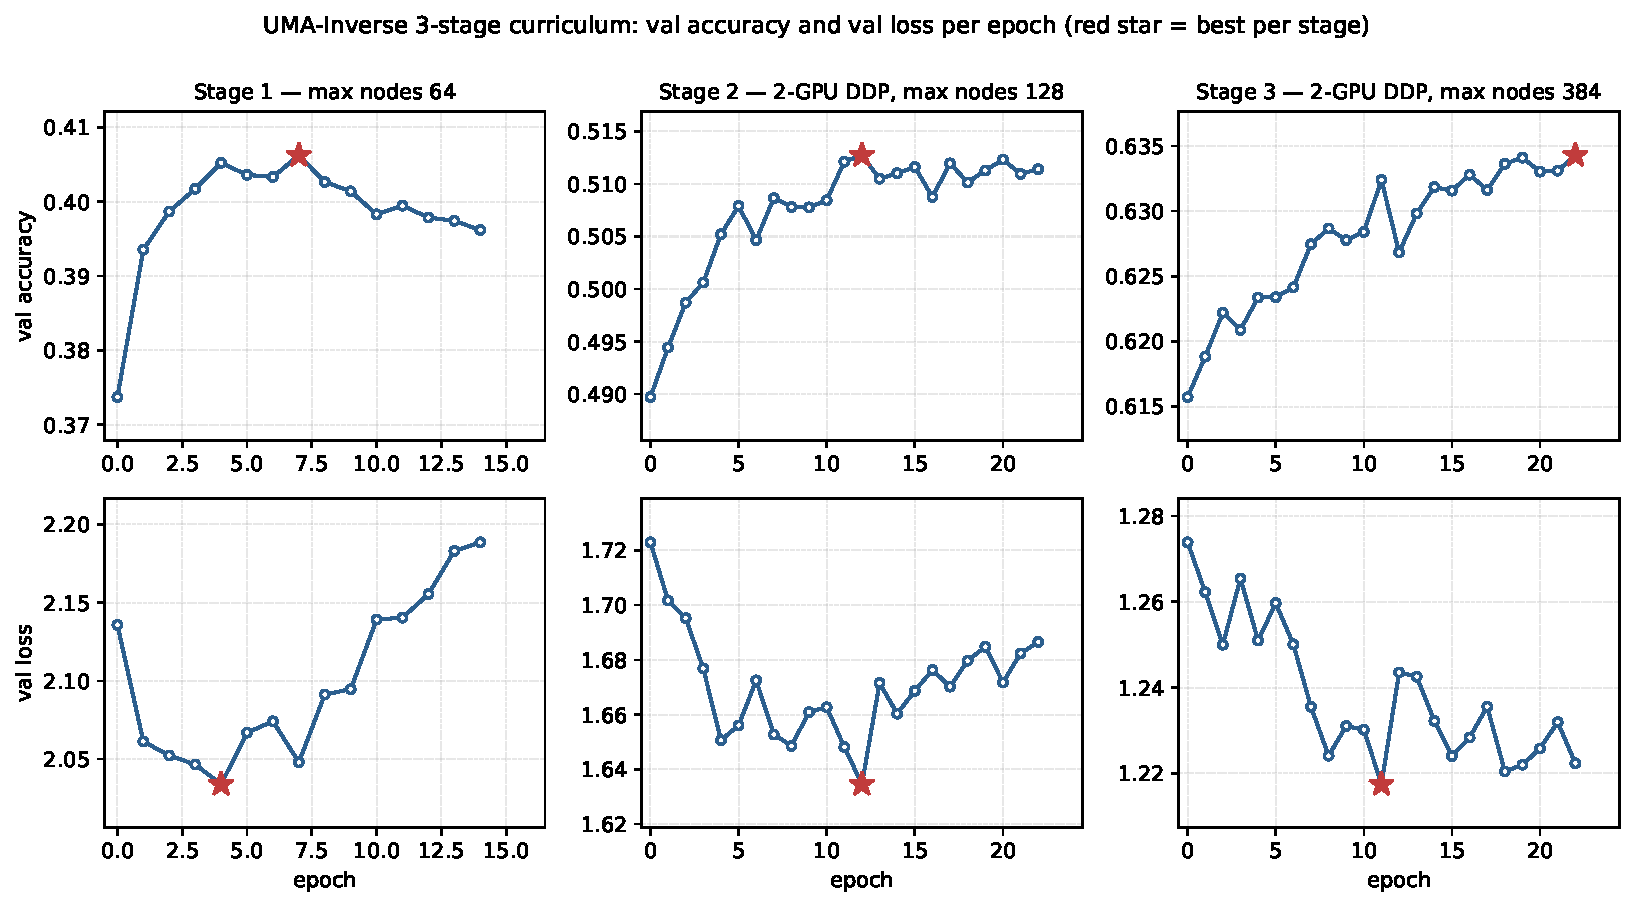
\includegraphics[width=\linewidth]{figures/fig4_training.pdf}
  \caption{\textbf{Three-stage training curves.} Validation accuracy and loss across the curriculum;
    the auxiliary distogram top-1 accuracy is overlaid for Stage 3. The best checkpoint (dashed line)
    is at epoch 11. \emph{[regenerate from v5 logs/csv]}}
  \label{fig:training}
\end{figure}

The model reaches validation accuracy 63.2\% at its best checkpoint, comparable to the
validation accuracy reported for LigandMPNN (${\sim}63.7\%$). The auxiliary distogram objective
trains to 93.1\% top-1 binned-distance accuracy, indicating the encoder's pair tensor is
strongly structure-predictive. We note (and report honestly) that the validation set here includes
nucleic-acid complexes routed into ligand context, making it a harder and broader set than
protein/small-molecule-only baselines.

\subsection{Teacher-forced sequence recovery}
\label{sec:results_tf}

On the full validation set, UMA-Inverse achieves 66.1\% per-PDB mean sequence recovery
(pooled 70.6\%) with perplexity 2.57 and expected calibration error (ECE)
0.0078. Per-amino-acid recovery is reported in Table~\ref{tab:peraacov}; as expected,
backbone-determined residues (Gly, Pro) recover most reliably. Zeroing the ligand features at
evaluation lowers mean recovery by $1.2$\,pp ($66.1\%\!\to\!64.8\%$) and native-sequence
log-likelihood by $0.083$\,nats/residue. Averaged over the whole protein this effect is modest---most
residues lie far from the ligand and are largely backbone-determined---but it concentrates near the
binding site, as the distance-shell analysis (\S\ref{sec:results_distal}) makes explicit.

\subsection{Interface sequence recovery}
\label{sec:results_iface}

\begin{figure}[t]
  \centering
  \begin{subfigure}[b]{0.48\linewidth}
    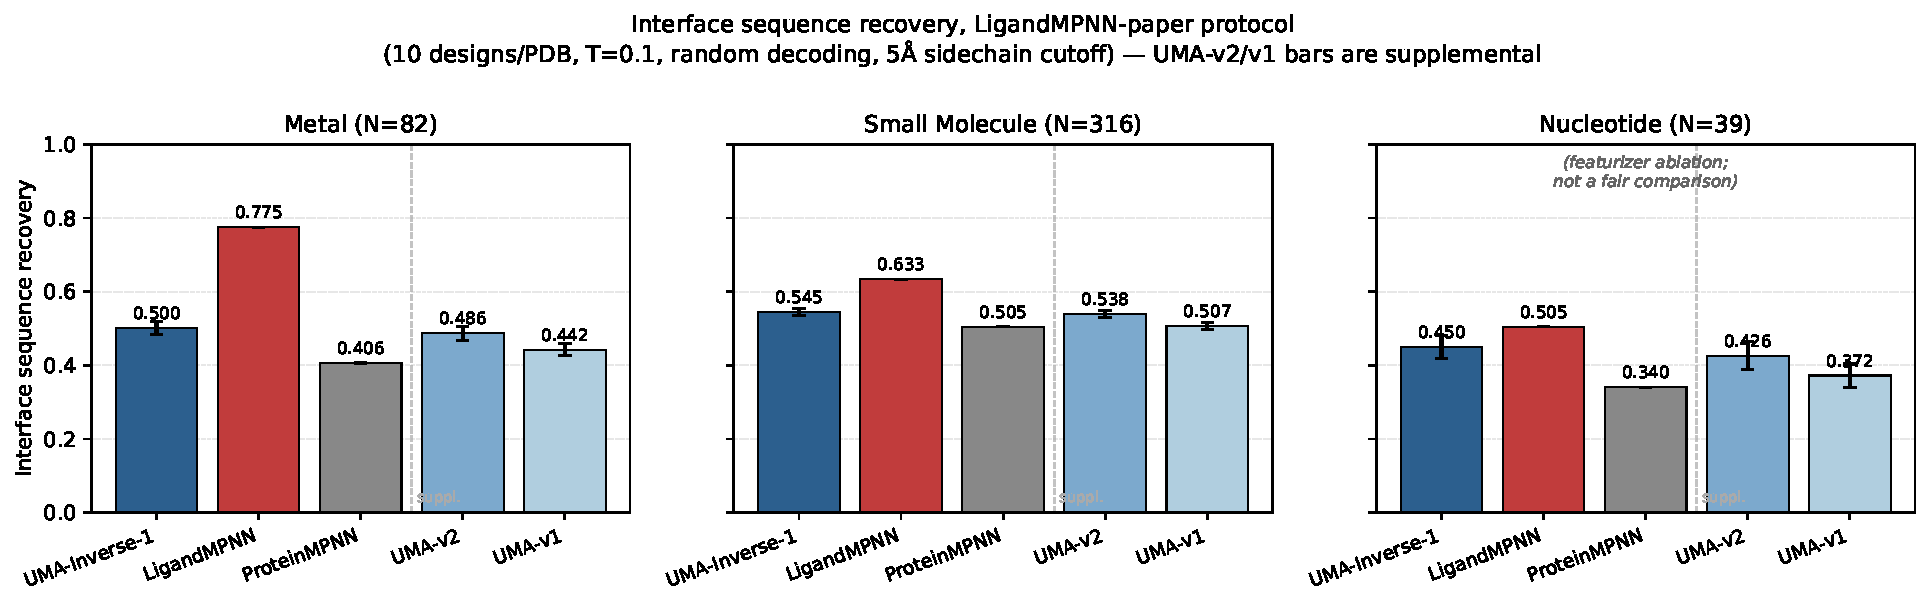
\includegraphics[width=\linewidth]{figures/fig2_benchmark_bars.pdf}
    \caption{Interface recovery by ligand class and model.}
    \label{fig:iface_bars}
  \end{subfigure}
  \hfill
  \begin{subfigure}[b]{0.48\linewidth}
    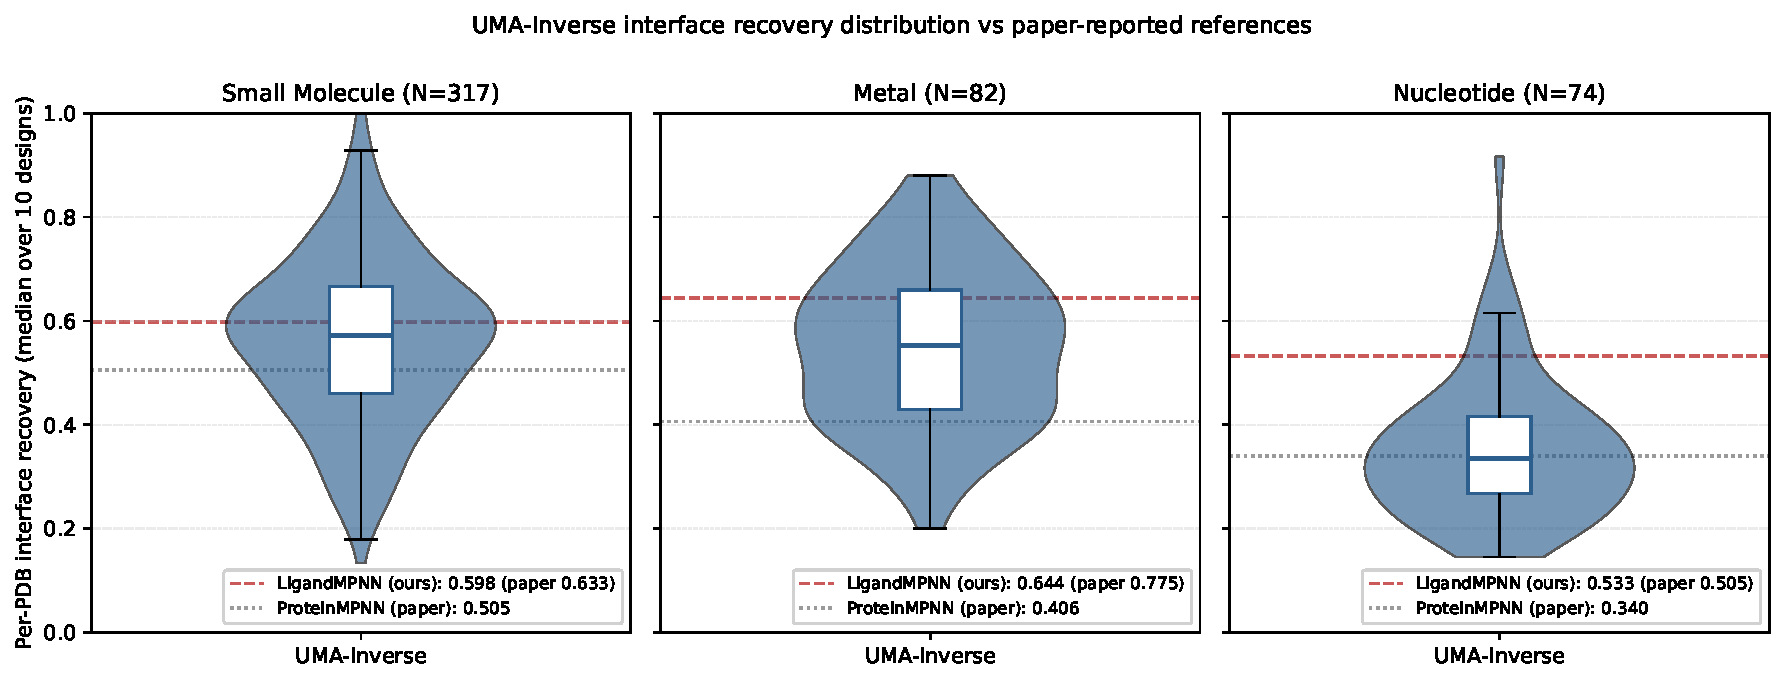
\includegraphics[width=\linewidth]{figures/fig3_violins.pdf}
    \caption{Per-PDB recovery distribution.}
    \label{fig:iface_violins}
  \end{subfigure}
  \caption{\textbf{Interface sequence recovery on the LigandMPNN test splits.}
    (a) Mean-of-per-PDB-medians for UMA-Inverse vs.\ our matched-protocol LigandMPNN run (LigandMPNN's
    published value in parentheses) and the published ProteinMPNN lower bound. (b) Per-PDB recovery
    distributions, with our matched LigandMPNN (dashed) and published ProteinMPNN (dotted) as
    references.}
  \label{fig:iface}
\end{figure}

We evaluate on all three LigandMPNN test splits (Table~\ref{tab:iface}). Because published baselines
depend on protocol details, we also re-run LigandMPNN ourselves on the identical structures under our
exact protocol (same $5$\,{\AA} interface mask, $10$ samples, mean-of-per-PDB-medians) and treat that
matched run as the controlled comparison. Under it, UMA-Inverse trails LigandMPNN by $3.7$\,pp on
small molecule ($56.1\%$ vs.\ $59.8\%$), $9.3$\,pp on metal ($55.1\%$ vs.\ $64.4\%$), and $18.0$\,pp on
nucleotide ($35.3\%$ vs.\ $53.3\%$); restricting both models to the exact same scored PDBs leaves the
gaps essentially unchanged ($4.1$/$9.0$/$17.7$\,pp). Notably, our matched LigandMPNN numbers are
\emph{lower} than its published values ($0.633$/$0.775$/$0.505$)---most strikingly on metal ($0.644$
vs.\ $0.775$)---so the gap is markedly smaller under a controlled comparison than the published numbers
imply; we report both, published values in parentheses. ProteinMPNN (no ligand conditioning, published)
is a lower bound ($0.505$/$0.406$/$0.471$). Both protein-comparable splits improve over the v3
predecessor (small molecule $54.5\%\!\to\!56.1\%$, metal $50.0\%\!\to\!55.1\%$). The nucleotide split
is, to our knowledge, the first such comparison for this model line, and here the result is frankly
\textbf{negative}: at $35.3\%$ UMA-Inverse falls not only below LigandMPNN but below the
ligand-agnostic ProteinMPNN ($47.1\%$). That is, routing the nucleic acid into the model makes it
\emph{worse} than ignoring ligand context entirely---the opposite of the small-molecule and metal
splits, where conditioning clearly helps (UMA-Inverse exceeds ProteinMPNN by $5.6$ and $14.5$\,pp).
We attribute this to a representational mismatch: a nucleic acid is a macromolecule (typically
$400$--$1500$ heavy atoms in these complexes), but the fixed-size ligand-atom context retains only
$50$, so the model is fed a small, unrepresentative fragment of the polymer. Treating nucleic acids as
compact ligands is the wrong abstraction; a dedicated macromolecular representation is required
(\S\ref{sec:discussion}).

\begin{table}[h]
\centering
\caption{Interface sequence recovery on the LigandMPNN test splits. Protocol: 10 autoregressive
  samples per PDB, $T{=}0.1$, random order, 5\,{\AA} sidechain--nonprotein cutoff; mean-of-per-PDB-medians.
  \textbf{LigandMPNN is re-run by us under this identical protocol on the same structures} (its
  published value from \citet{dauparas2023atomic} in parentheses); LigandMPNN (this work) is scored on
  $300$/$72$/$67$ of the PDBs after excluding cases where its parsed native sequence disagreed with
  ours. ProteinMPNN is the published value.}
\label{tab:iface}
\begin{tabular}{lcccc}
\toprule
Split & N & UMA-Inverse & LigandMPNN & ProteinMPNN \\
               &     &             & ours (paper) & (paper) \\
\midrule
Small molecule & 317 & 0.561 & 0.598 (0.633) & 0.505 \\
Metal          & 82  & 0.551 & 0.644 (0.775) & 0.406 \\
Nucleotide     & 74  & 0.353 & 0.533 (0.505) & 0.471 \\
\bottomrule
\end{tabular}
\end{table}

\subsection{Pocket-fixed design and cofolding}
\label{sec:results_pocket}

\begin{figure}[t]
  \centering
  \begin{subfigure}[b]{0.48\linewidth}
    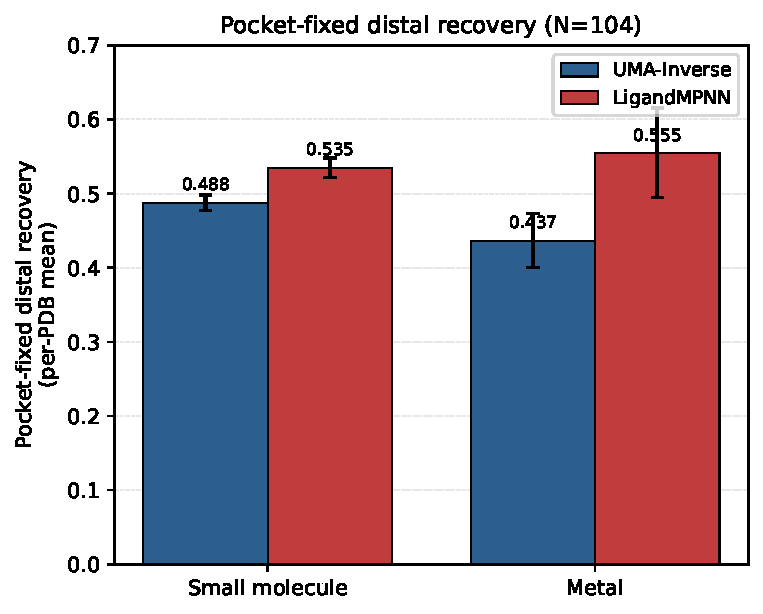
\includegraphics[width=\linewidth]{figures/fig5_pocket_distal.pdf}
    \caption{Pocket-fixed distal recovery by ligand class.}
  \end{subfigure}
  \hfill
  \begin{subfigure}[b]{0.48\linewidth}
    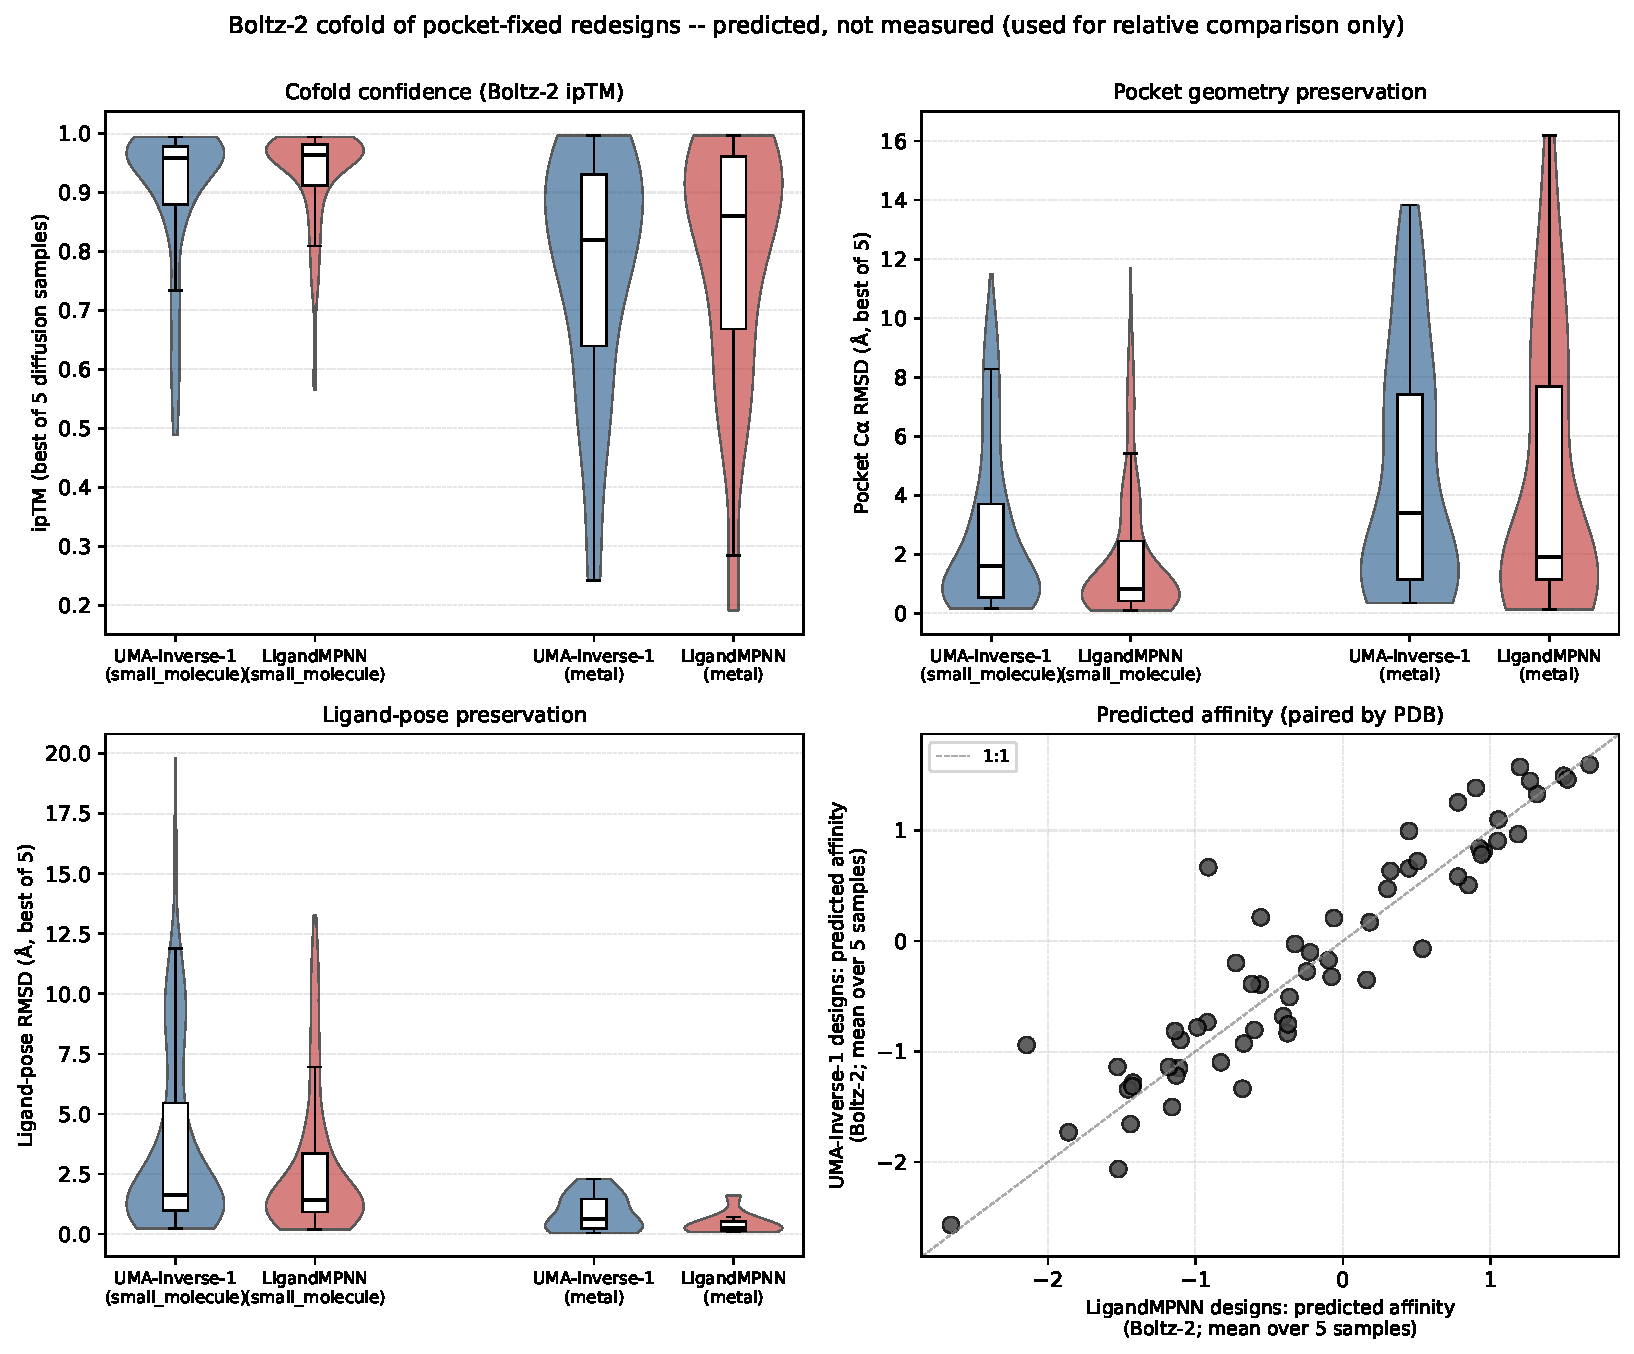
\includegraphics[width=\linewidth]{figures/fig6_cofold.pdf}
    \caption{Boltz-2 cofold: ligand-pose RMSD vs.\ native and LigandMPNN.}
  \end{subfigure}
  \caption{\textbf{Constrained (pocket-fixed) design.} (a)~With the native pocket held fixed, both
    methods redesign the distal positions; LigandMPNN recovers them somewhat better than UMA-Inverse
    ($N{=}104$). (b)~Boltz-2 cofold ligand-pose RMSD for the native sequence, UMA-Inverse, and
    LigandMPNN: both design methods sit near the native floor and are confidently folded (ligand
    ipTM $\approx$$0.96$), with LigandMPNN modestly closer to the native pose (paired Wilcoxon
    $p{=}0.003$, $N{=}86$).}
  \label{fig:pocket}
\end{figure}

This setting mirrors a common real design task: rather than redesigning the catalytic or binding
pocket, the known pocket is held fixed---preserving its established activity---while the rest of the
protein is redesigned (Fig.~\ref{fig:pocket}). Over $104$ targets with the pocket fixed to native
identity, LigandMPNN recovers more of the distal (non-pocket) positions than UMA-Inverse
($53.7\%$ vs.\ $48.3\%$ overall; small molecule $53.5\%$ vs.\ $48.8\%$, metal $55.5\%$ vs.\ $43.7\%$),
mirroring the interface-recovery gap. At a matched sampling temperature ($T{=}0.1$) UMA-Inverse's
designs are also less diverse (mean pairwise Hamming $0.14$ vs.\ $0.19$); we report this only with the
caveat that diversity is temperature-tunable and a single nominal temperature is not directly
comparable across models, so it is not a controlled comparison.

Because native-sequence recovery penalizes any valid non-native solution---it assumes the crystal
sequence is the unique optimum, which it is not---we also validate the designs structurally, an
orthogonal check that makes no such assumption. We cofold each design with Boltz-2
\citep{Passaro2025.06.14.659707} and compare, under the identical protocol, against the native crystal
sequence (an upper bound on agreement) and LigandMPNN. Across $104$ targets (ligand pose measurable on
$86$ after heavy-atom matching), UMA-Inverse redesigns are confidently folded and
ligand-binding-competent: ligand ipTM $\approx$$0.96$ and a median best-of-5 ligand-pose RMSD of
$1.53$\,{\AA}, within $\sim$$0.6$\,{\AA} of the native-sequence floor ($0.90$\,{\AA}). They do not,
however, match LigandMPNN's geometry: LigandMPNN is modestly but significantly better on ligand pose
($1.27$\,{\AA} median; paired $\Delta{=}{+}0.13$\,{\AA}, Wilcoxon $p{=}0.003$, $N{=}86$), and likewise
on pocket-C$\alpha$ and whole-scaffold RMSD. The cofold thus confirms UMA-Inverse produces foldable,
ligand-competent redesigns but does not overturn LigandMPNN's accuracy advantage.

\subsection{Distogram representation and ligand-distal signal}
\label{sec:results_distal}

\begin{figure}[t]
  \centering
  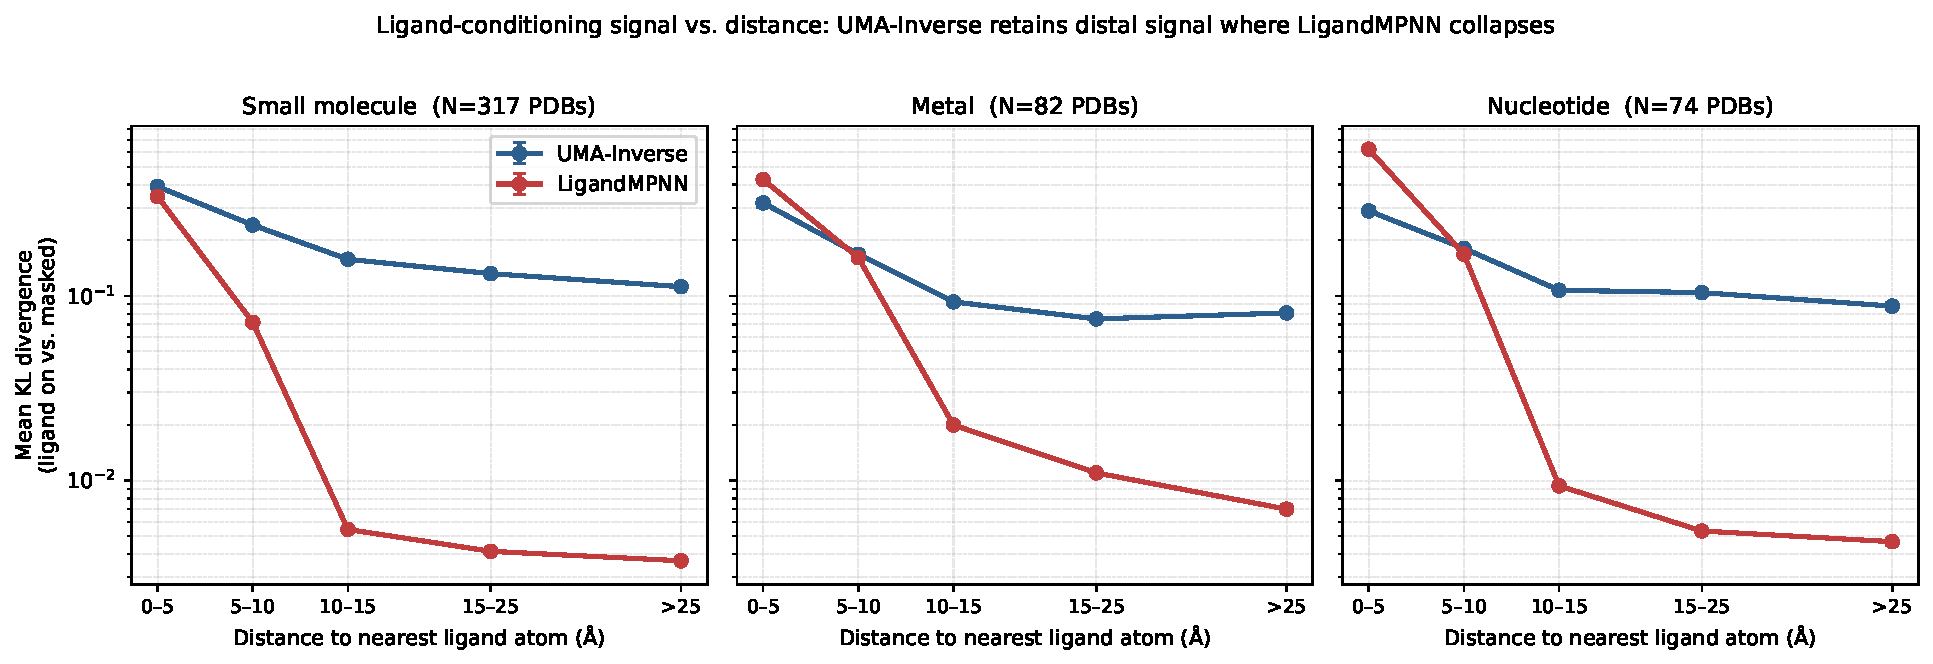
\includegraphics[width=\linewidth]{figures/fig7_distal_signal.pdf}
  \caption{\textbf{Ligand-conditioning signal vs.\ distance, by ligand class.} Mean KL divergence
    between the ligand-conditioned and ligand-masked per-residue distributions in 5\,{\AA} shells
    (log scale, $\pm$1 SEM), for UMA-Inverse and LigandMPNN on the small-molecule ($N{=}317$), metal
    ($N{=}82$), and nucleotide ($N{=}74$) test splits. Both respond at the immediate interface, but
    beyond $\sim$$10$\,{\AA} LigandMPNN's signal collapses toward zero while UMA-Inverse retains a
    substantial signal---the dense pair encoder propagates ligand identity to distal residues.}
  \label{fig:distal}
\end{figure}

The auxiliary distogram head recovers binned inter-residue distances at 93.1\% top-1 accuracy,
confirming the encoder maintains an explicit geometric representation. To probe how far ligand
information reaches, we measure---in 5\,{\AA} distance shells---the KL divergence between each model's
per-residue amino-acid distribution with the ligand present versus masked (Fig.~\ref{fig:distal}).
At the immediate interface ($0$--$5$\,{\AA}) both models are strongly ligand-sensitive; LigandMPNN is
in fact the more sensitive on the metal and nucleotide splits. The two diverge sharply with distance:
beyond $10$\,{\AA} LigandMPNN's signal falls to near zero (mean KL $\le 0.02$ at $10$--$15$\,{\AA} for
all three classes), whereas UMA-Inverse retains a substantial signal ($0.09$--$0.16$ at that shell)
that persists past $25$\,{\AA}---several-fold, up to $\sim$$30\times$, LigandMPNN's at distal shells.
This \emph{distal persistence} is a representational property of the dense, all-pairs PairMixer
encoder: ligand identity is made available throughout the fold rather than confined to the binding
pocket as a local message-passing graph confines it. We are careful not to over-read it---this signal
does \emph{not} translate into a design advantage, as LigandMPNN is more accurate both at the interface
(\S\ref{sec:results_iface}) and on pocket-fixed distal positions (\S\ref{sec:results_pocket}). What it
shows is a concrete, measurable difference in \emph{what the architecture encodes}; whether global
ligand propagation helps would have to be tested on tasks where distal context matters beyond
single-position native recovery---allosteric or multi-site design, or function- rather than
identity-based objectives---which we leave to future work.

% -----------------------------------------------------------------------
\section{Discussion}
\label{sec:discussion}

UMA-Inverse shows that a compact ($\sim$$3.3$M-parameter), MSA-free, distogram-supervised dense pair
encoder---without triangle attention or a sequence track---is a viable architecture for
ligand-conditioned inverse folding: it trains on commodity GPUs, reaches within $4$--$9$\,pp of
LigandMPNN on the small-molecule and metal splits, and produces confidently folded,
ligand-binding-competent sequences. It does not, however, match LigandMPNN, which is more accurate on
interface recovery, on pocket-fixed distal recovery, and on cofolded ligand pose; and its
nucleic-acid routing is an outright negative result (below the ligand-agnostic baseline), as a
macromolecular partner does not fit the compact-ligand representation. We therefore present
UMA-Inverse as a compact baseline and as the vehicle for one specific, reproducible finding---how a
dense all-pairs encoder distributes ligand information through a fold---rather than as a
state-of-the-art design tool. A caveat on the primary metric itself: native-sequence recovery rewards
reproducing the crystal sequence and penalizes equally valid alternatives, so it understates any
method whose designs are foldable but non-native; our cofold analysis is the orthogonal check, and by
it both methods yield valid complexes (LigandMPNN modestly closer to the native pose).

\paragraph{What the auxiliary distogram and ligand attention buy.}
The two architectural additions target distinct failure modes. The distogram objective constrains the
encoder to keep its pair tensor structure-predictive (93.1\% top-1), rather than collapsing
it into a sequence-only shortcut; the learned ligand attention then reads that tensor in a
position-specific way, repairing the distal-residue divergence of a uniform mean-pool. We motivate
these choices by design rationale and the auxiliary head's high top-1 binned-distance accuracy
rather than a controlled on/off ablation.

\paragraph{Remaining gaps.}
Against our matched-protocol LigandMPNN, the metal and small-molecule gaps are modest under this
controlled comparison ($55.1\%$ vs.\ $64.4\%$ and $56.1\%$ vs.\ $59.8\%$) and smaller than LigandMPNN's
published numbers imply. The nucleotide split is the clear failure: at $35.3\%$ UMA-Inverse falls below
even the ligand-agnostic ProteinMPNN ($47.1\%$), so its nucleic-acid conditioning is net-negative. We
read this as a representational mismatch rather than undertraining---the same model \emph{benefits} from
small-molecule and metal context, but a nucleic acid is a macromolecule of hundreds to over a thousand
heavy atoms, of which the fixed-size ligand-atom context retains only $50$, so the model is conditioned
on an unrepresentative fragment. For the protein-ligand splits we lack a controlled ablation isolating
the architectural source of the residual gaps, and so do not attribute them to a specific cause. We also
observe mild late-training calibration drift (validation
cross-entropy rising while accuracy plateaus), suggesting early stopping by validation loss---rather
than accuracy---is the correct checkpoint-selection criterion, which we adopt.

\paragraph{Future directions.}
The most direct follow-up to our results is to test whether the encoder's distal ligand propagation
confers any practical advantage on tasks where distal context plausibly matters---allosteric or
multi-site design, or function- rather than identity-based objectives---since it demonstrably does not
help single-position native recovery. A controlled, temperature-matched recovery-vs-diversity (Pareto)
comparison against LigandMPNN would also place the diversity question on firmer footing than the
single-temperature snapshot reported here. The nucleotide failure motivates a \emph{dedicated
macromolecular representation} for nucleic acids---e.g.\ nucleotide-level tokens or a separate
NA track---rather than forcing a polymer through a fixed-size compact-ligand atom context. Other
extensions include flow-matching~\citep{lipman2022flow} in place of cross-entropy, full RDKit-derived
ligand chemistry and bond topology (scaffolded but disabled in this model), and adding triangle
self-attention to the pair encoder.

% -----------------------------------------------------------------------
\section{Conclusion}

We introduced UMA-Inverse, a ligand- and nucleic-acid-conditioned inverse-folding model that replaces
sparse GNN message-passing with a distogram-supervised dense pair encoder and a learned
ligand-attention decoder. Trained on commodity GPUs using the public LigandMPNN data split, the model
achieves 66.1\% teacher-forced recovery and 56.1\%/55.1\%/35.3\%
interface recovery on the small-molecule/metal/nucleotide splits, with confidently folded,
ligand-binding-competent cofolds. It does not surpass LigandMPNN on recovery or cofolded pose, and its
nucleic-acid routing is a negative result (below the ligand-agnostic baseline---a macromolecule is the
wrong fit for a compact-ligand context). Its contribution is to show that a compact, MSA-free,
distogram-supervised dense pair encoder is a viable alternative architecture for small-molecule and
metal partners, and to characterize its distinctive propagation of ligand information to residues far
beyond the binding pocket.

\paragraph{Code and data availability.}
Code, the trained checkpoint, and evaluation scripts are released at
\href{https://github.com/WSobo/UMA-Inverse-2}{\texttt{github.com/WSobo/UMA-Inverse-2}}. The LigandMPNN
training split is available at
\href{https://github.com/dauparas/LigandMPNN}{\texttt{github.com/dauparas/LigandMPNN}}.

\paragraph{Acknowledgments.}
Training compute was provided by the Yeh Laboratory at UC Santa Cruz.
% [add advisor acknowledgment here]

% -----------------------------------------------------------------------
\appendix

\section{Per-amino-acid recovery}
\label{sec:aa_recovery}

Per-amino-acid teacher-forced recovery on the full validation set (875 PDBs, 525{,}224 residues),
with native and predicted marginal frequencies for reference (Table~\ref{tab:peraacov}). Recovery is
highest for backbone-constrained residues (Pro 0.953, Gly 0.906) and lowest for low-frequency,
context-dependent residues (Gln 0.497, Met 0.500); predicted and native compositions track closely.

\begin{table}[h]
\centering
\caption{Per-amino-acid teacher-forced recovery, native frequency, and predicted frequency on the
  full validation set. UMA-Inverse / v5, best checkpoint (epoch 11).}
\label{tab:peraacov}
\begin{tabular}{lccc@{\hskip 2em}lccc}
\toprule
AA & Recovery & Native & Pred. & AA & Recovery & Native & Pred. \\
\midrule
A & 0.737 & 0.084 & 0.083 & M & 0.500 & 0.020 & 0.012 \\
C & 0.610 & 0.012 & 0.009 & N & 0.606 & 0.042 & 0.036 \\
D & 0.716 & 0.059 & 0.065 & P & 0.953 & 0.047 & 0.061 \\
E & 0.657 & 0.067 & 0.074 & Q & 0.497 & 0.036 & 0.022 \\
F & 0.687 & 0.041 & 0.037 & R & 0.609 & 0.051 & 0.047 \\
G & 0.906 & 0.072 & 0.080 & S & 0.651 & 0.059 & 0.062 \\
H & 0.553 & 0.024 & 0.016 & T & 0.673 & 0.053 & 0.057 \\
I & 0.693 & 0.057 & 0.054 & V & 0.769 & 0.072 & 0.079 \\
K & 0.603 & 0.056 & 0.055 & W & 0.592 & 0.015 & 0.011 \\
L & 0.814 & 0.097 & 0.107 & Y & 0.645 & 0.035 & 0.032 \\
\bottomrule
\end{tabular}
\end{table}

\section{Validation metrics by training stage}
\label{sec:training_detail}

\begin{table}[h]
\centering
\caption{Final validation metrics at the end of each curriculum stage (UMA-Inverse / v5 run).}
\label{tab:training_stages}
\begin{tabular}{lccccc}
\toprule
Stage & GPUs & Max nodes & Best epoch & Val accuracy & Val loss \\
\midrule
Stage 1 & 1$\times$A5500 & 64  & 4  & 40.5\% & 2.034 \\
Stage 2 & 2$\times$A100  & 128 & 12 & 51.3\% & 1.635 \\
Stage 3 & 2$\times$A100  & 384 & 11 & 63.2\% & 1.217 \\
\bottomrule
\end{tabular}
\end{table}

% -----------------------------------------------------------------------
\bibliographystyle{unsrtnat}
\bibliography{references}

\end{document}
